\documentclass[journal]{IEEEtran}

\usepackage{amsmath,amssymb}
\usepackage{booktabs}
\usepackage{graphicx}
\usepackage{cite}
\usepackage{url}
\usepackage[section]{placeins}

\renewcommand\IEEEkeywordsname{Keywords}

\title{Terrain-Aware Multi-Objective Optimization of Campus Wireless Backhaul Links Using Link-Budget Modeling and Radio Mobile Validation}

\author{Simeon~Nsabiyumva$^{1*}$,
Samuel~Babalola$^{1}$,
David~Tuyishimire$^{1}$,
and~Isaac~Museveni$^{1}$\\
$^{1}$Faculty of Software Engineering, African Leadership University, Kigali, Rwanda\\
Emails: snsabiyumva@alueducation.com, s.babalola@alustudent.com, dtuyishimire@alueducation.com, imuseveni@alueducation.com\\
$^{*}$Corresponding author}

\begin{document}

\maketitle

\begin{abstract}
Campus backhaul links are often planned from link-budget calculations and then adjusted after terrain simulation. This paper develops a terrain-aware planning model that selects antenna height and antenna gain for a point-to-point 5.8 GHz campus backhaul link while satisfying received-signal and fade-margin constraints. The model combines free-space path loss with terrain and statistical correction terms calibrated from Radio Mobile simulations. A 30-scenario matrix was generated for a 7.159 km link between the Nyarugenge and Remera campus sites using antenna heights from 5 m to 30 m and antenna gains from 10 dBi to 24 dBi. The Radio Mobile results show fade margins from 0.23 dB to 53.68 dB, with 23 of 30 scenarios satisfying a 20 dB margin and 13 of 30 satisfying a 30 dB margin. Free-space path loss alone produced a received-signal MAE of 8.337 dB against Radio Mobile. Adding an average terrain/statistical correction reduced the MAE to 6.574 dB, while a height-calibrated correction reduced the MAE to 0.043 dB. Under the normalized deployment-burden objective used in this study, the minimum-cost feasible design is 5 m and 10 dBi for a 20 dB margin, and 5 m and 16 dBi for a 30 dB margin. The results show that antenna height should not be selected by a monotonic ``higher is better'' rule when the terrain obstruction term changes with height.
\end{abstract}

\begin{IEEEkeywords}
wireless backhaul, link budget, terrain-aware propagation, Radio Mobile, antenna height optimization, fade margin, campus network planning
\end{IEEEkeywords}

\section{Introduction}

Point-to-point wireless backhaul remains useful for campus, institutional, and community networks because it can connect separated sites without leased fiber or trenching. Microwave backhaul is widely used where optical fiber is expensive, slow, or impractical to deploy, but it requires careful treatment of line-of-sight, Fresnel-zone clearance, and local obstruction effects \cite{brown2023planning}. The engineering decision is therefore practical as well as analytical: choose a permitted frequency, antenna height, antenna gain, transmit power, and receiver threshold that produce enough fade margin without unnecessary tower height or equipment cost.

Analytical link-budget calculations provide a clear first estimate by combining transmit power, antenna gains, cable losses, receiver sensitivity, and path loss. However, free-space path loss assumes an unobstructed path and does not capture terrain obstruction, reflection, diffraction, clutter, or Fresnel-zone behavior on its own \cite{rappaport2002wireless,molisch2011wireless}. Terrain-aware tools such as Radio Mobile add path-profile and statistical propagation effects, but the tool output still has to be translated into an equipment recommendation. This paper studies that decision layer.

The study uses a corrected 7.159 km campus link between the Nyarugenge and Remera sites. Radio Mobile simulations were run at 5825 MHz for 30 antenna-height and antenna-gain combinations. This frequency is treated as the account-permitted high-frequency test case, while lower-frequency TV White Space operation is discussed only as a planning alternative because the Radio Mobile account used in the experiment rejected a direct 600 MHz run. The analytical model was then compared against the Radio Mobile received-signal and fade-margin outputs.

The contributions are:
\begin{itemize}
    \item a link-budget optimization model for campus point-to-point backhaul planning;
    \item a terrain-aware correction structure that separates free-space loss from terrain, obstruction, and statistical losses;
    \item a Radio Mobile validation matrix over six antenna heights and five antenna gains;
    \item a deployment-burden comparison that identifies the minimum-cost feasible antenna configuration under 20 dB and 30 dB fade-margin thresholds.
\end{itemize}

\section{Related Work}

Recent propagation-modeling work confirms that received-signal and path-loss prediction remain central to wireless planning. Vasudevan and Yuksel survey machine-learning methods for radio propagation modeling and show that environment-aware features are increasingly used for path-loss and coverage prediction \cite{vasudevan2024machine}. Yapar et al. describe a pathloss radio-map prediction challenge, emphasizing evaluation methodology for environment-aware propagation prediction \cite{yapar2024overview}. These works motivate terrain-sensitive modeling, but their main focus is radio-map or machine-learning prediction rather than equipment selection for a point-to-point campus backhaul link.

Terrain remains a major source of modeling error. Soo et al. study radio propagation over uneven terrain and show that uneven profiles can change propagation behavior compared with flat-surface assumptions \cite{soo2025radio}. Fernandez et al. develop a dual-slope path-loss model for urban and suburban vehicular sensing, reinforcing the need for empirical corrections beyond a single free-space estimate \cite{fernandez2024dual}.

Optimization is also established in wireless planning. Antenna-positioning work has used genetic algorithms for coverage improvement \cite{callesesteban2024optimizing}, and backhaul topology studies have used optimization for network-level design \cite{hernandez2024spectral,khaturia2019efficient}. TV White Space research also continues to address spectrum and regulatory constraints for wider-area connectivity \cite{cunha2025impact,mach2023improved}. Radio Mobile itself has been evaluated for line-of-sight paths using terrain datasets \cite{kaschel2019analysis}. The gap addressed here is narrower: a transparent link-budget decision model for selecting antenna height and gain, validated against Radio Mobile terrain-aware outputs for a campus-scale point-to-point backhaul link.

\section{Problem Statement}

Given two fixed campus sites, a permitted frequency band, a receiver sensitivity, and a required fade margin, the planning problem is to choose antenna height and antenna gain so that the link is feasible while deployment burden is minimized. The deployment burden represents practical cost pressure from mast height, antenna gain, transmit power, and frequency-band constraints.

The corrected sites used in the experiment are shown in Table~\ref{tab:sites}.
The table defines the fixed endpoints used by all simulations; therefore, changes in the later results come from antenna height and gain rather than from changing link distance or site location.

\begin{table}[!htbp]
\centering
\caption{Radio Mobile sites used in the experiment}
\label{tab:sites}
\begin{tabular}{lccc}
\toprule
Site & Latitude & Longitude & Elevation\\
\midrule
Nyarugenge & 45.703489 & 13.720818 & 57.70 m\\
Remera & 45.643370 & 13.753787 & 14.10 m\\
\bottomrule
\end{tabular}
\end{table}

\section{Analytical Model}

For candidate design $i$, the received signal is
\begin{equation}
P_{rx,i}=P_{t,i}+G_{t,i}+G_{r,i}-L_{t,i}-L_{r,i}-PL_{total,i},
\end{equation}
where $P_t$ is transmit power in dBm, $G_t$ and $G_r$ are antenna gains in dBi, $L_t$ and $L_r$ are line losses in dB, and $PL_{total}$ is total path loss in dB.

The maximum allowable path loss is
\begin{equation}
PL_{max,i}=P_{t,i}+G_{t,i}+G_{r,i}-L_{t,i}-L_{r,i}-P_{sens}-FM_{req}.
\end{equation}

The free-space path loss is
\begin{equation}
PL_{FS,i}=32.44+20\log_{10}(d_i)+20\log_{10}(f_i),
\end{equation}
with distance $d_i$ in km and frequency $f_i$ in MHz. The terrain-aware total path loss is modeled as
\begin{equation}
PL_{total,i}=PL_{FS,i}+L_{terrain,i}+L_{stat,i}+L_{clutter,i}+L_{impl,i}.
\end{equation}

Radio Mobile reports free-space loss, obstruction loss, forest loss, urban loss, statistical loss, total path loss, received signal, and fade margin. In this study the calibrated correction is
\begin{equation}
L_{corr,i}=PL_{RM,i}-PL_{FS,i},
\end{equation}
where $PL_{RM,i}$ is the Radio Mobile total path loss.

Fade margin is
\begin{equation}
FM_i=P_{rx,i}-P_{sens}.
\end{equation}
The feasibility constraint is
\begin{equation}
FM_i \ge FM_{req}.
\end{equation}

The deployment-burden objective used for ranking feasible designs is
\begin{equation}
\min C_i=w_h\frac{h_i}{h_{max}}+w_g\frac{G_i}{G_{max}},
\end{equation}
where $h_i$ is the common antenna height at both ends, $G_i$ is the common antenna gain at both ends, $h_{max}=30$ m, $G_{max}=24$ dBi, $w_h=0.55$, and $w_g=0.45$. Height is weighted slightly more than gain because mast height usually carries civil-work, permission, and safety costs.

\section{Radio Mobile Methodology}

The experiment used the saved Nyarugenge and Remera sites in the Radio Mobile account. The frequency was 5825 MHz because the account accepted this WiFi band. A direct 600 MHz TVWS trial was rejected by the account, so no 600 MHz result is reported.

The fixed radio settings were:
\begin{itemize}
    \item transmit power: 0.1 W, equivalent to 20 dBm;
    \item transmitter line loss: 1 dB;
    \item receiver line loss: 1 dB;
    \item receiver threshold: 0.5 $\mu$V, equivalent to approximately -113.02 dBm;
    \item required reliability: 70\%;
    \item land cover: enabled;
    \item two-ray option: enabled.
\end{itemize}

The simulation matrix used antenna heights of 5, 10, 15, 20, 25, and 30 m. Antenna gains were 10, 12, 16, 19, and 24 dBi. The same height and gain were used at both ends in each run, giving 30 scenarios.

\section{Results}

The results are organized in the same order as the planning decision: first the path-loss behavior by height is summarized, then the feasible fade-margin design space is shown, and finally the received-signal trend is used to confirm the same terrain-driven pattern.

Table~\ref{tab:heightloss} shows that the Radio Mobile terrain-sensitive loss is not monotonic with antenna height. Each row aggregates scenarios with the same height, and gain is not shown because Radio Mobile's obstruction and statistical losses stayed constant across gain for a fixed height. The 20 m case has the largest obstruction loss and the weakest received signal, while the 10 m and 30 m cases have the lowest total path loss. This table is important because it explains why the recommended deployment is not simply the tallest mast.

\begin{table}[!htbp]
\centering
\caption{Radio Mobile path-loss components by antenna height}
\label{tab:heightloss}
\begin{tabular}{rrrr}
\toprule
Height (m) & Obstruction (dB) & Statistical (dB) & Total PL (dB)\\
\midrule
5 & -3.18 & 6.54 & 129.16\\
10 & -5.87 & 6.54 & 125.48\\
15 & 1.71 & 6.55 & 133.06\\
20 & 19.43 & 6.55 & 150.79\\
25 & 3.89 & 6.56 & 135.25\\
30 & -6.02 & 6.56 & 125.34\\
\bottomrule
\end{tabular}
\end{table}

The fade-margin heatmap in Fig.~\ref{fig:heatmap} summarizes feasibility across the 30 scenarios. It is not strictly necessary because the same values can be described in text and in the line plot, but it is useful as a compact design map: a planner can immediately see which height-gain pairs pass a required margin. Overall, 23 scenarios satisfy a 20 dB fade-margin threshold and 13 scenarios satisfy a 30 dB threshold.

\begin{figure}[!htbp]
\centering
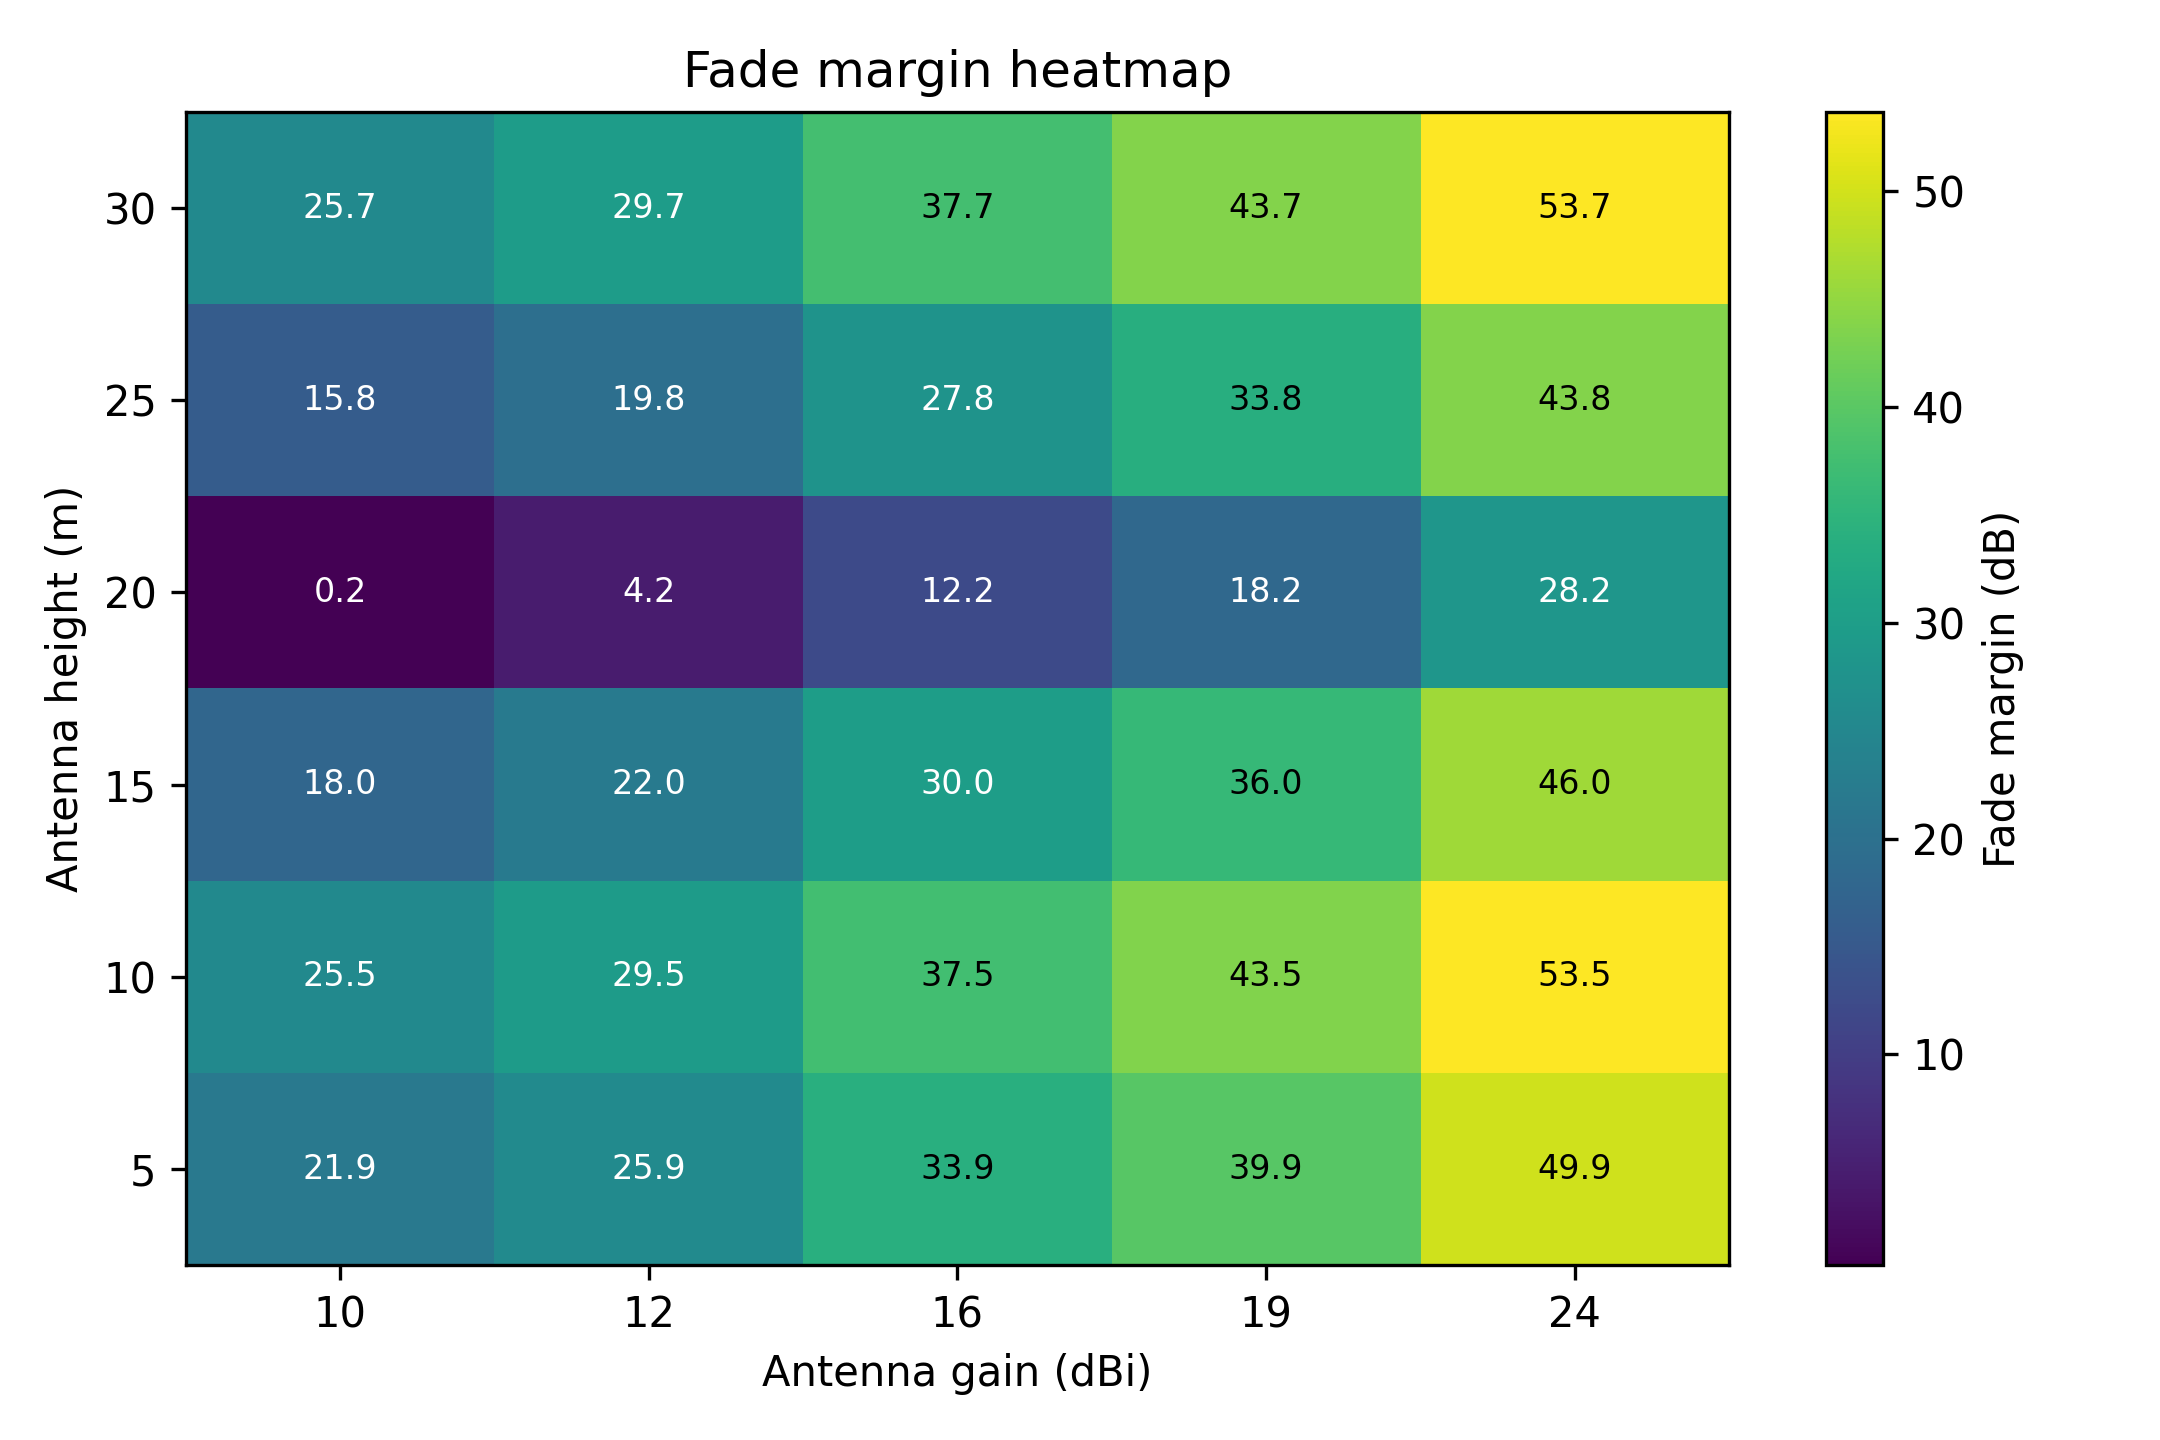
\includegraphics[width=\linewidth]{figures/fade_margin_heatmap.png}
\caption{Fade margin over antenna height and antenna gain at 5825 MHz.}
\label{fig:heatmap}
\end{figure}

Fig.~\ref{fig:fadeheight} shows that increasing gain improves margin at every height, but increasing height does not always improve margin. This behavior comes from the Radio Mobile obstruction term, not from the free-space component, because distance and frequency are fixed.

\begin{figure}[!htbp]
\centering
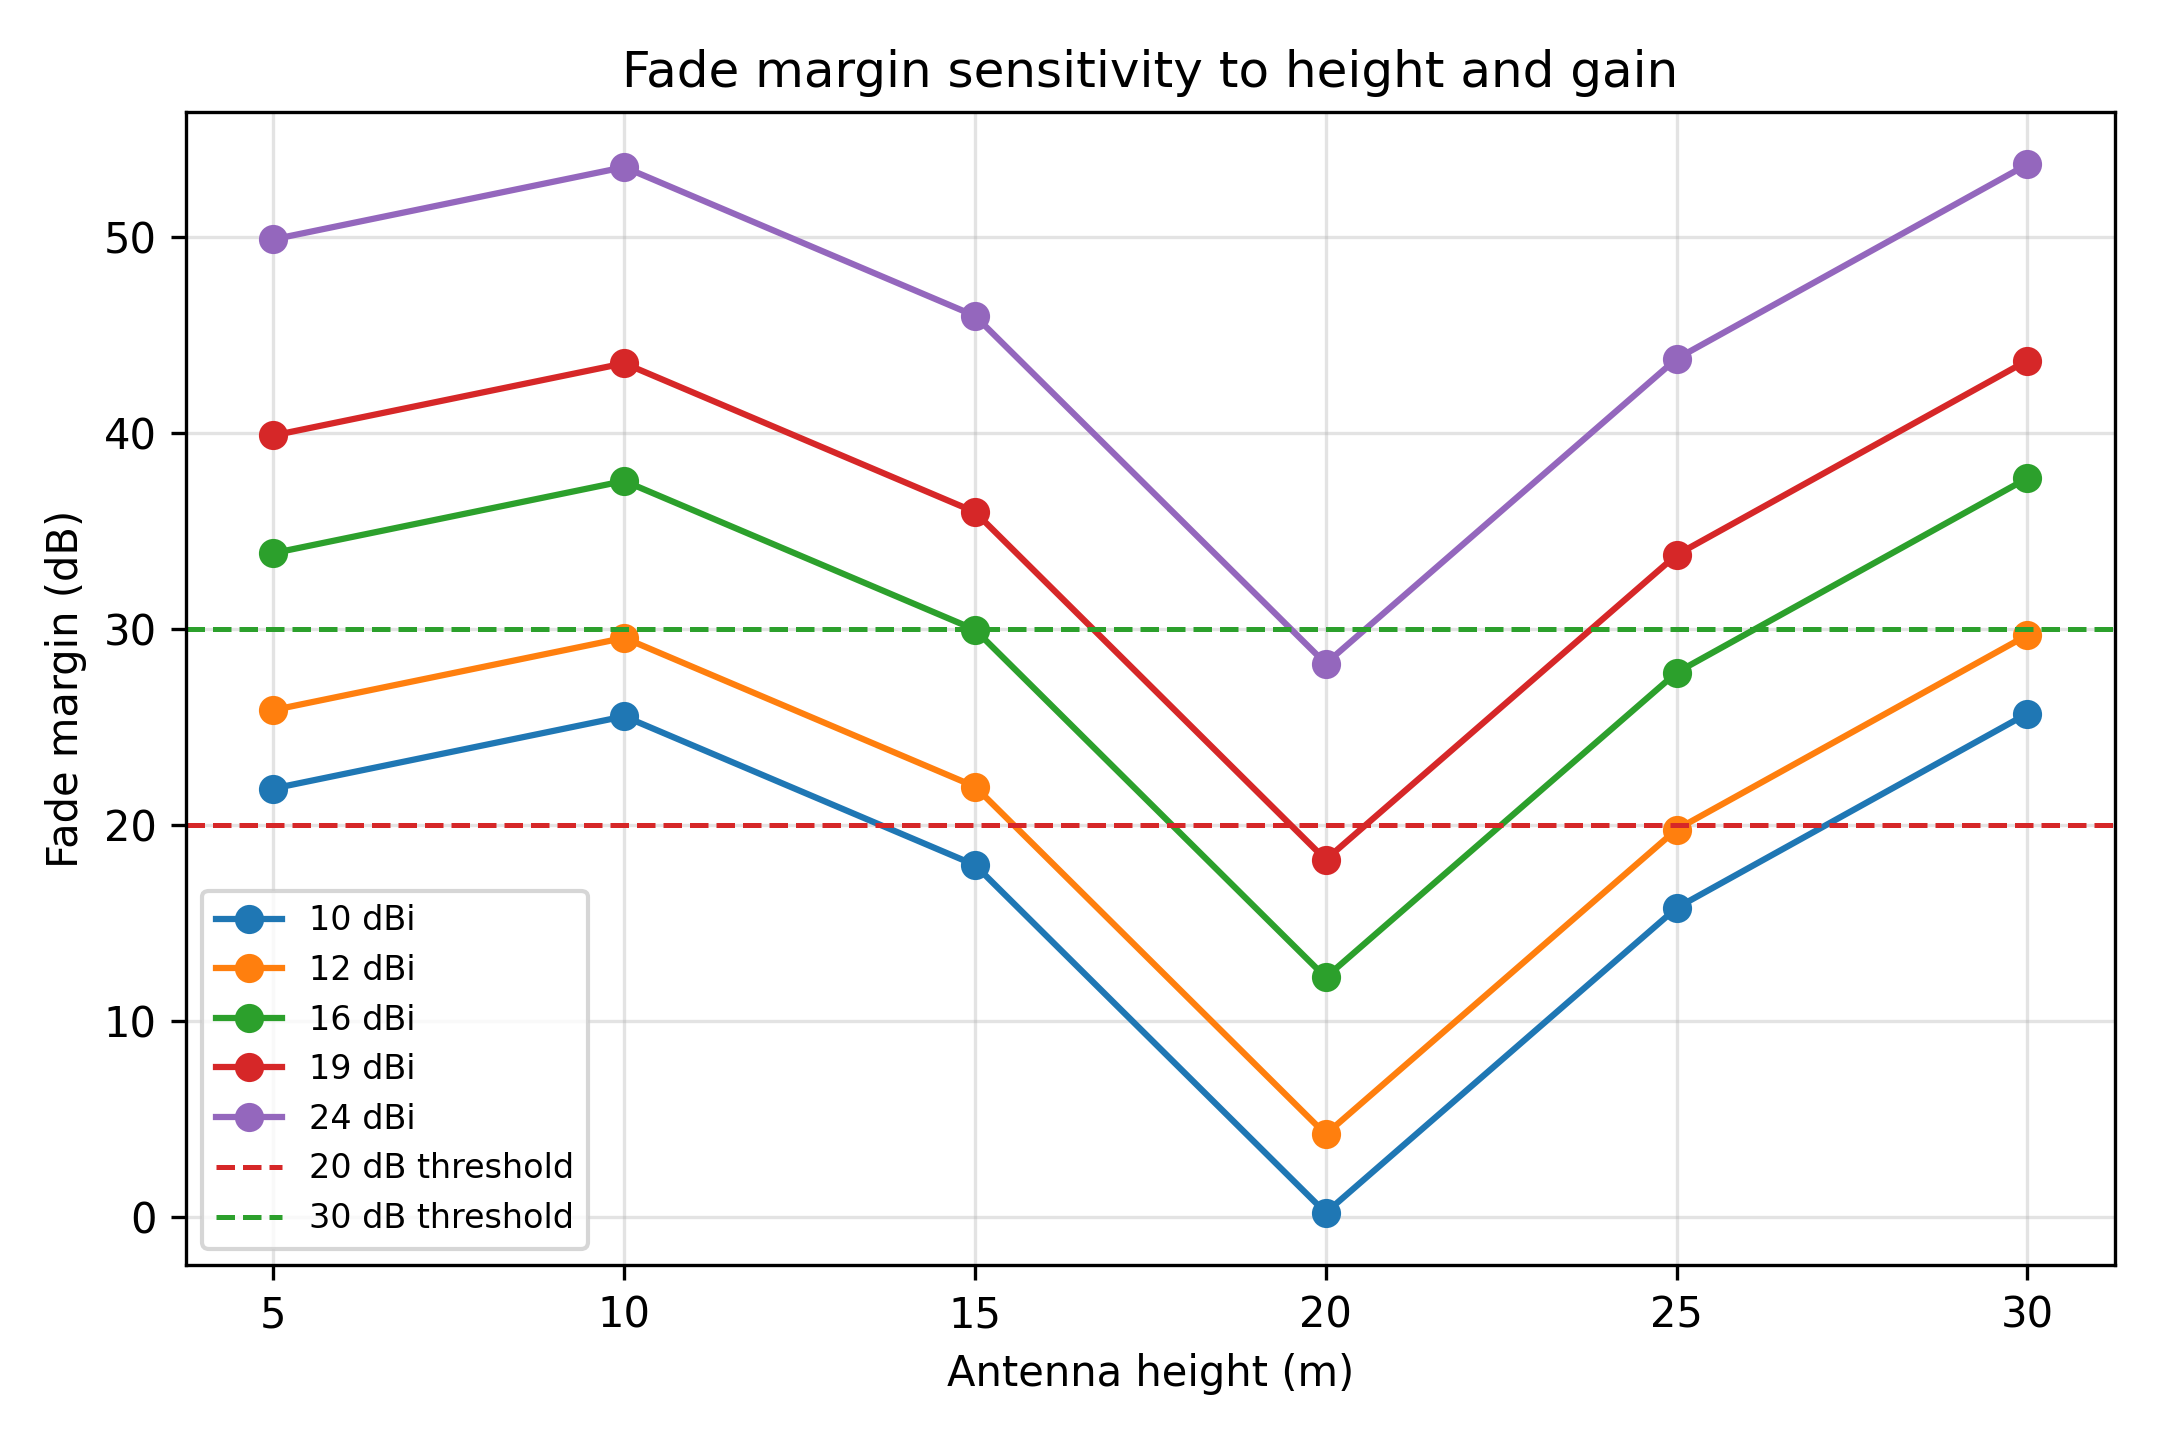
\includegraphics[width=\linewidth]{figures/fade_margin_vs_height.png}
\caption{Fade margin as a function of antenna height for each antenna gain.}
\label{fig:fadeheight}
\end{figure}

Fig.~\ref{fig:rxheight} presents the same terrain effect from the received-signal point of view. The strongest received levels occur at 10 m and 30 m, while the 20 m case is weakest because of the higher obstruction loss. Including both fade margin and received signal is useful because fade margin directly supports feasibility decisions, whereas received signal shows the physical link-budget output before subtracting the receiver threshold.

\begin{figure}[!htbp]
\centering
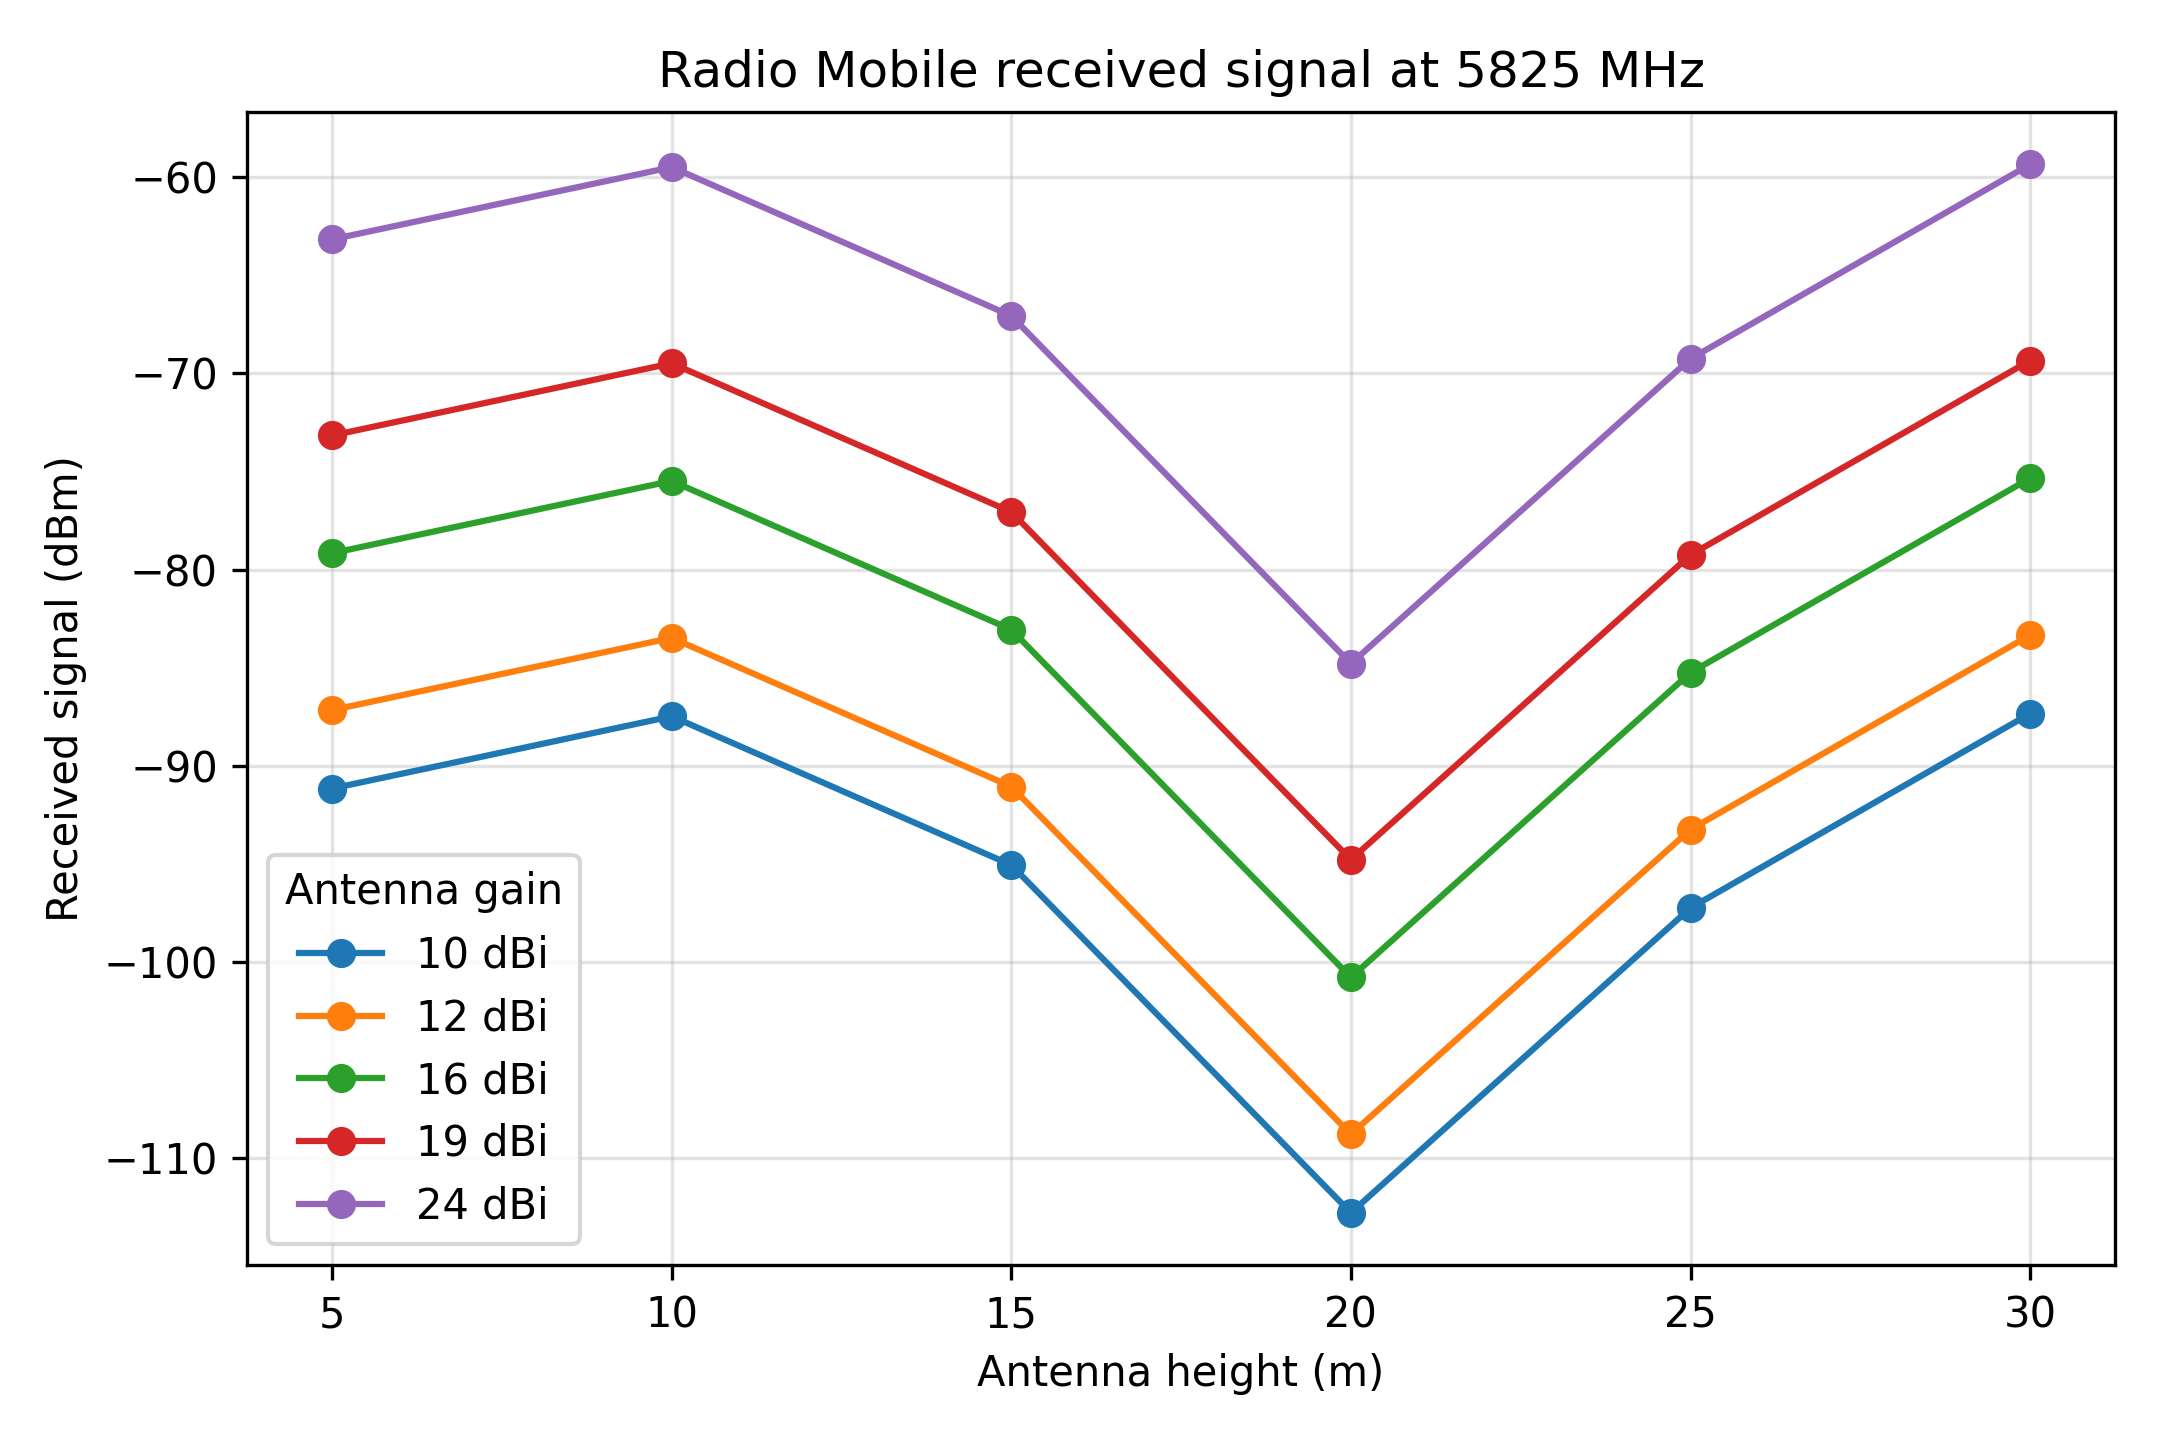
\includegraphics[width=\linewidth]{figures/received_signal_vs_height.png}
\caption{Radio Mobile received signal as a function of antenna height for each antenna gain.}
\label{fig:rxheight}
\end{figure}

\section{Model Validation}

Three analytical models were compared against the Radio Mobile received signal:
\begin{itemize}
    \item FSPL only;
    \item FSPL plus the average terrain/statistical correction;
    \item FSPL plus a height-calibrated correction.
\end{itemize}

The error metrics are shown in Table~\ref{tab:validation}. The table compares three analytical assumptions and reports both numerical error and feasibility agreement under 20 dB and 30 dB fade-margin requirements. The FSPL-only model has an MAE of 8.337 dB and an RMSE of 12.030 dB. The average-correction model reduces MAE to 6.574 dB. The height-calibrated correction reduces MAE and RMSE to 0.043 dB because Radio Mobile's terrain and statistical losses are constant across gain for a fixed height in this experiment. This result should be interpreted as simulation calibration, not field validation.

\begin{table}[!htbp]
\centering
\caption{Analytical model validation against Radio Mobile}
\label{tab:validation}
\scriptsize
\setlength{\tabcolsep}{2pt}
\begin{tabular}{lccccc}
\toprule
Model & Req. & MAE & RMSE & FM MAE & Agree\\
 & (dB) & Rx & Rx & (dB) & \\
\midrule
FSPL only & 20 & 8.337 & 12.030 & 8.337 & 0.767\\
FSPL only & 30 & 8.337 & 12.030 & 8.337 & 0.633\\
FSPL + avg. corr. & 20 & 6.574 & 8.673 & 6.574 & 0.767\\
FSPL + avg. corr. & 30 & 6.574 & 8.673 & 6.574 & 0.833\\
FSPL + height corr. & 20 & 0.043 & 0.043 & 0.043 & 1.000\\
FSPL + height corr. & 30 & 0.043 & 0.043 & 0.043 & 1.000\\
\bottomrule
\end{tabular}
\end{table}

Fig.~\ref{fig:error} shows the prediction error by antenna height. The FSPL-only model misses the height-dependent obstruction behavior. The height-calibrated model tracks Radio Mobile closely because the correction is estimated from the same height-specific simulation outputs.

\begin{figure}[!htbp]
\centering
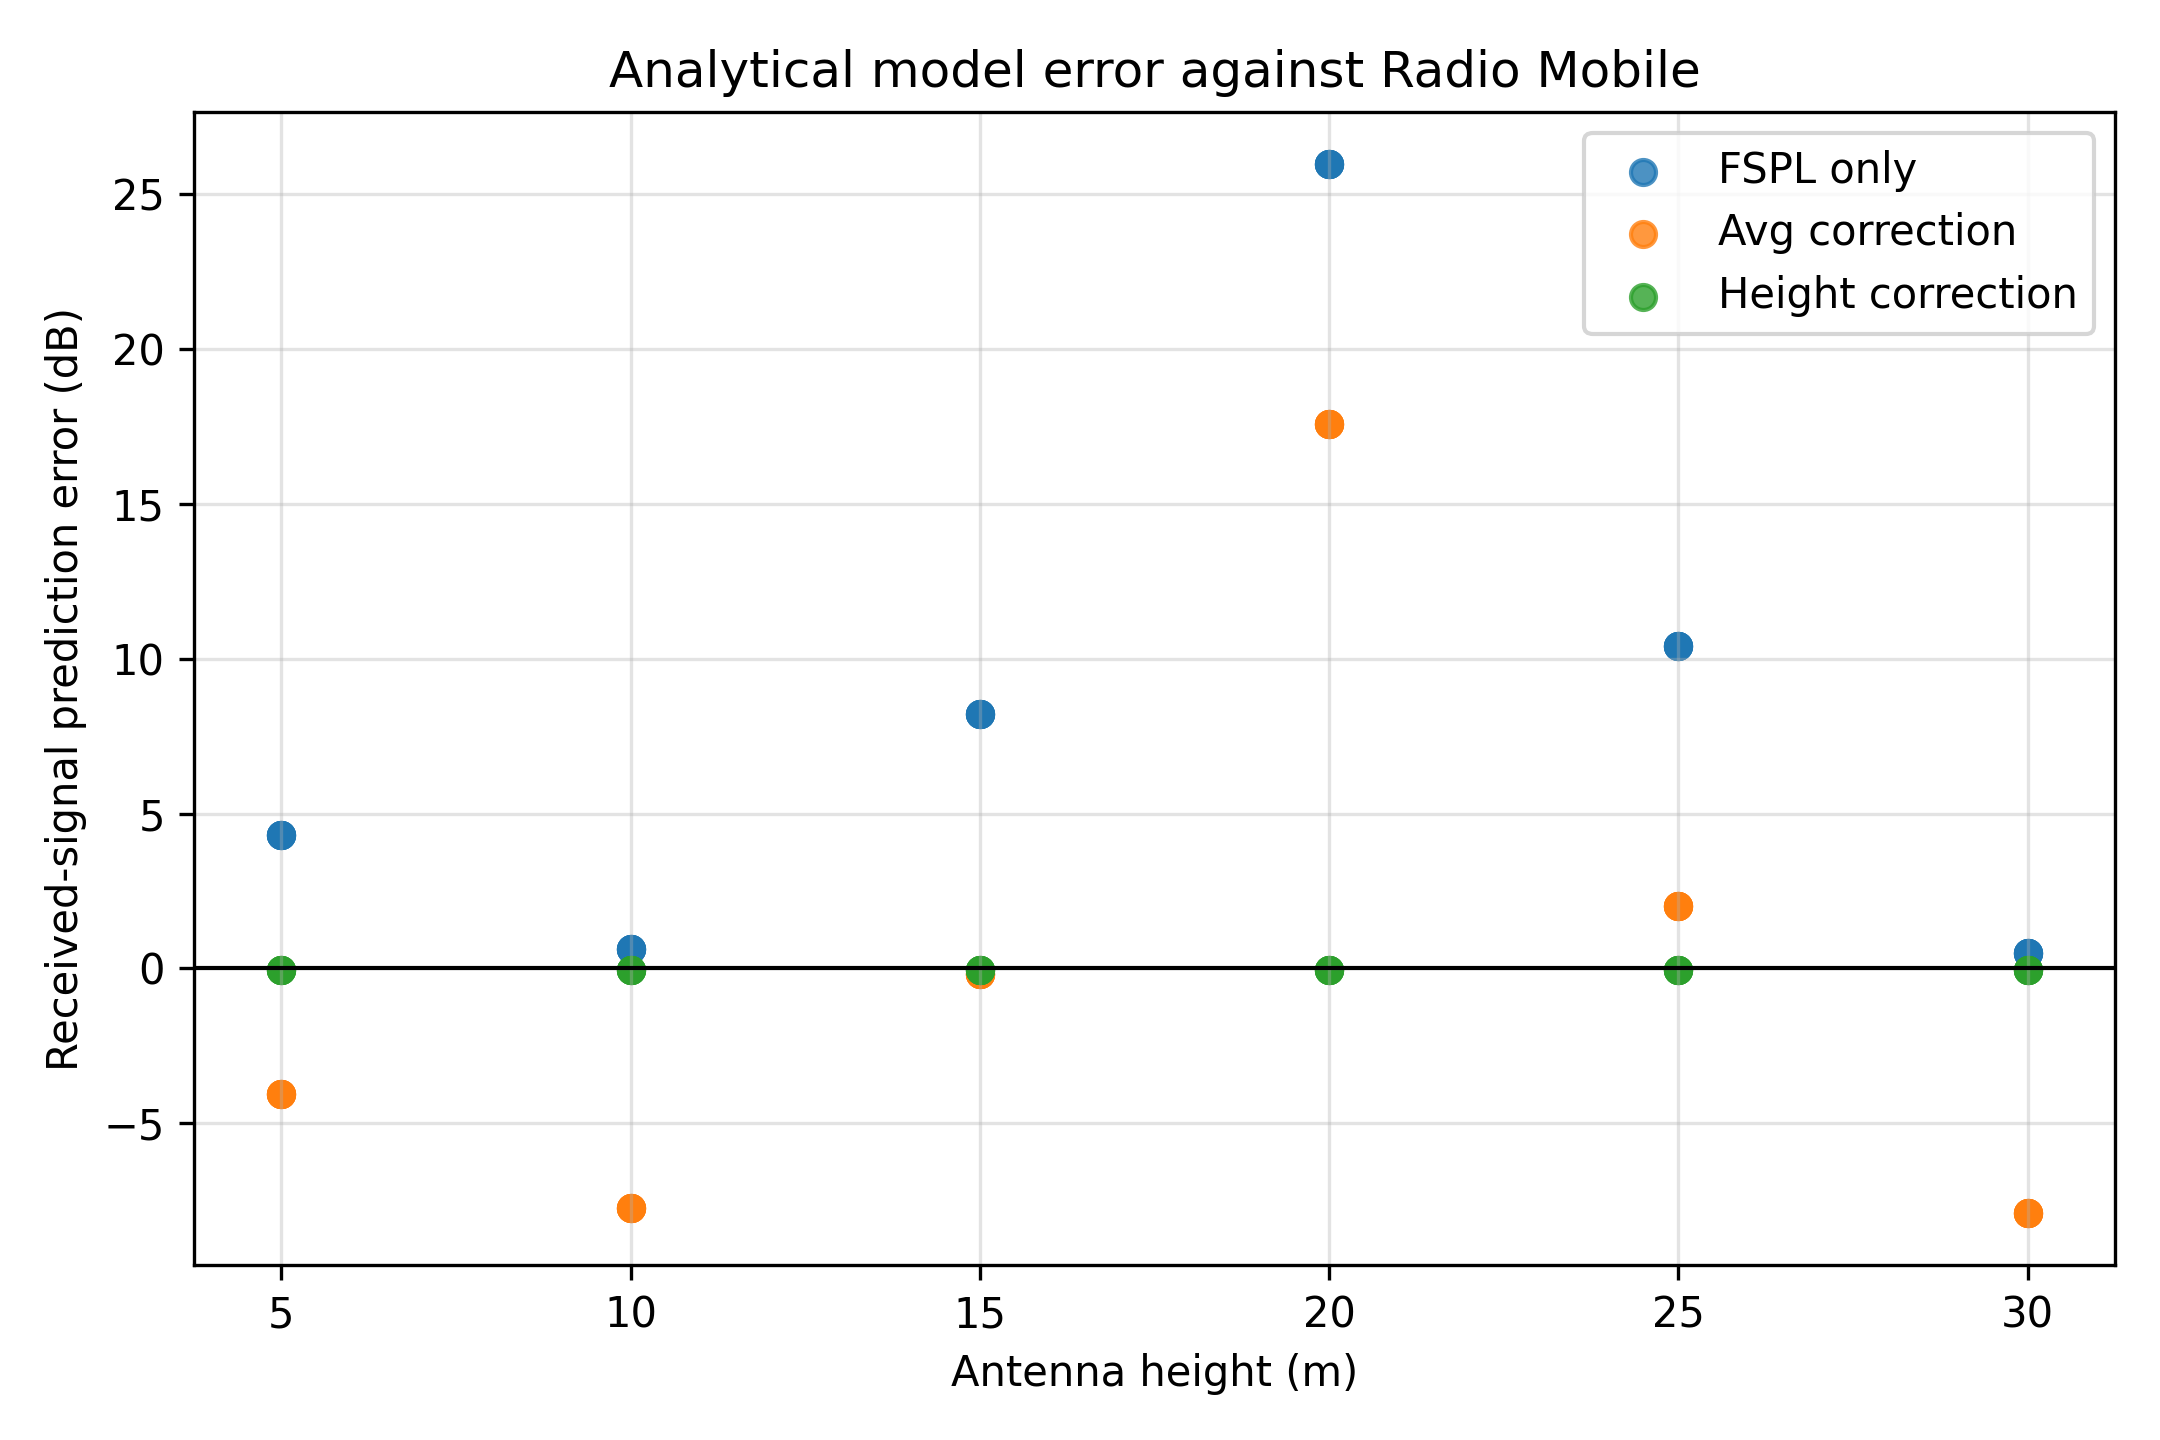
\includegraphics[width=\linewidth]{figures/model_error_by_height.png}
\caption{Received-signal prediction error against Radio Mobile.}
\label{fig:error}
\end{figure}

\section{Deployment Planning}

The deployment plan follows the practical sequence recommended in deployment-planning guidance: estimate demand, calculate the link budget, simulate the path with terrain data, select equipment, perform a site survey, install and align the link, and monitor performance after commissioning. For this campus link, the purpose is a point-to-point backhaul connection between Nyarugenge and Remera rather than general access coverage.

The planned service should first be translated into a target throughput and reliability requirement. The Radio Mobile experiment used a 70\% reliability setting and evaluated 20 dB and 30 dB fade-margin thresholds. A 20 dB margin is acceptable for a cost-conscious campus bridge, while the 30 dB case is recommended when the link will carry critical traffic or when seasonal rain, rooftop clutter, or future interference are expected to reduce the margin.

The selected radio configuration is a symmetric 5.8 GHz outdoor bridge with 20 dBm transmit power, 1 dB cable loss at each end, and directional antennas. The baseline deployment is 5 m mounting height and 10 dBi gain, which gives 21.86 dB fade margin and is the minimum-burden design satisfying the 20 dB target. The conservative deployment is 5 m mounting height and 16 dBi gain, which gives 33.86 dB fade margin and satisfies the 30 dB target without increasing mast height. The 20 m height should be avoided for this specific path because Radio Mobile reports a 19.43 dB obstruction loss at that height.

Before installation, both rooftops should be surveyed to confirm safe mast locations, cable routing, power availability, grounding, lightning protection, and clear antenna pointing toward the opposite site. The installer should verify azimuth and tilt from the Radio Mobile profile, mount the radios with short low-loss cable runs, align the dishes using received-signal readings, and record the final RSSI, noise floor, modulation rate, throughput, latency, and packet loss. After commissioning, the link should be monitored for fade-margin changes, interference, and traffic growth so that antenna gain, channel selection, or a lower-frequency alternative can be reconsidered if the measured margin drops below the planning target.

\section{Deployment Recommendation}

The normalized deployment-burden objective selects 5 m and 10 dBi as the minimum-cost feasible design for a 20 dB fade-margin target. This case gives a Radio Mobile fade margin of 21.86 dB. For a more conservative 30 dB target, the selected design is 5 m and 16 dBi, giving a fade margin of 33.86 dB.

Fig.~\ref{fig:cost} shows the deployment-burden tradeoff. The 20 m scenarios are unattractive because the obstruction loss is high, so even larger antenna gain gives limited benefit compared with lower-height alternatives.

\begin{figure}[!htbp]
\centering
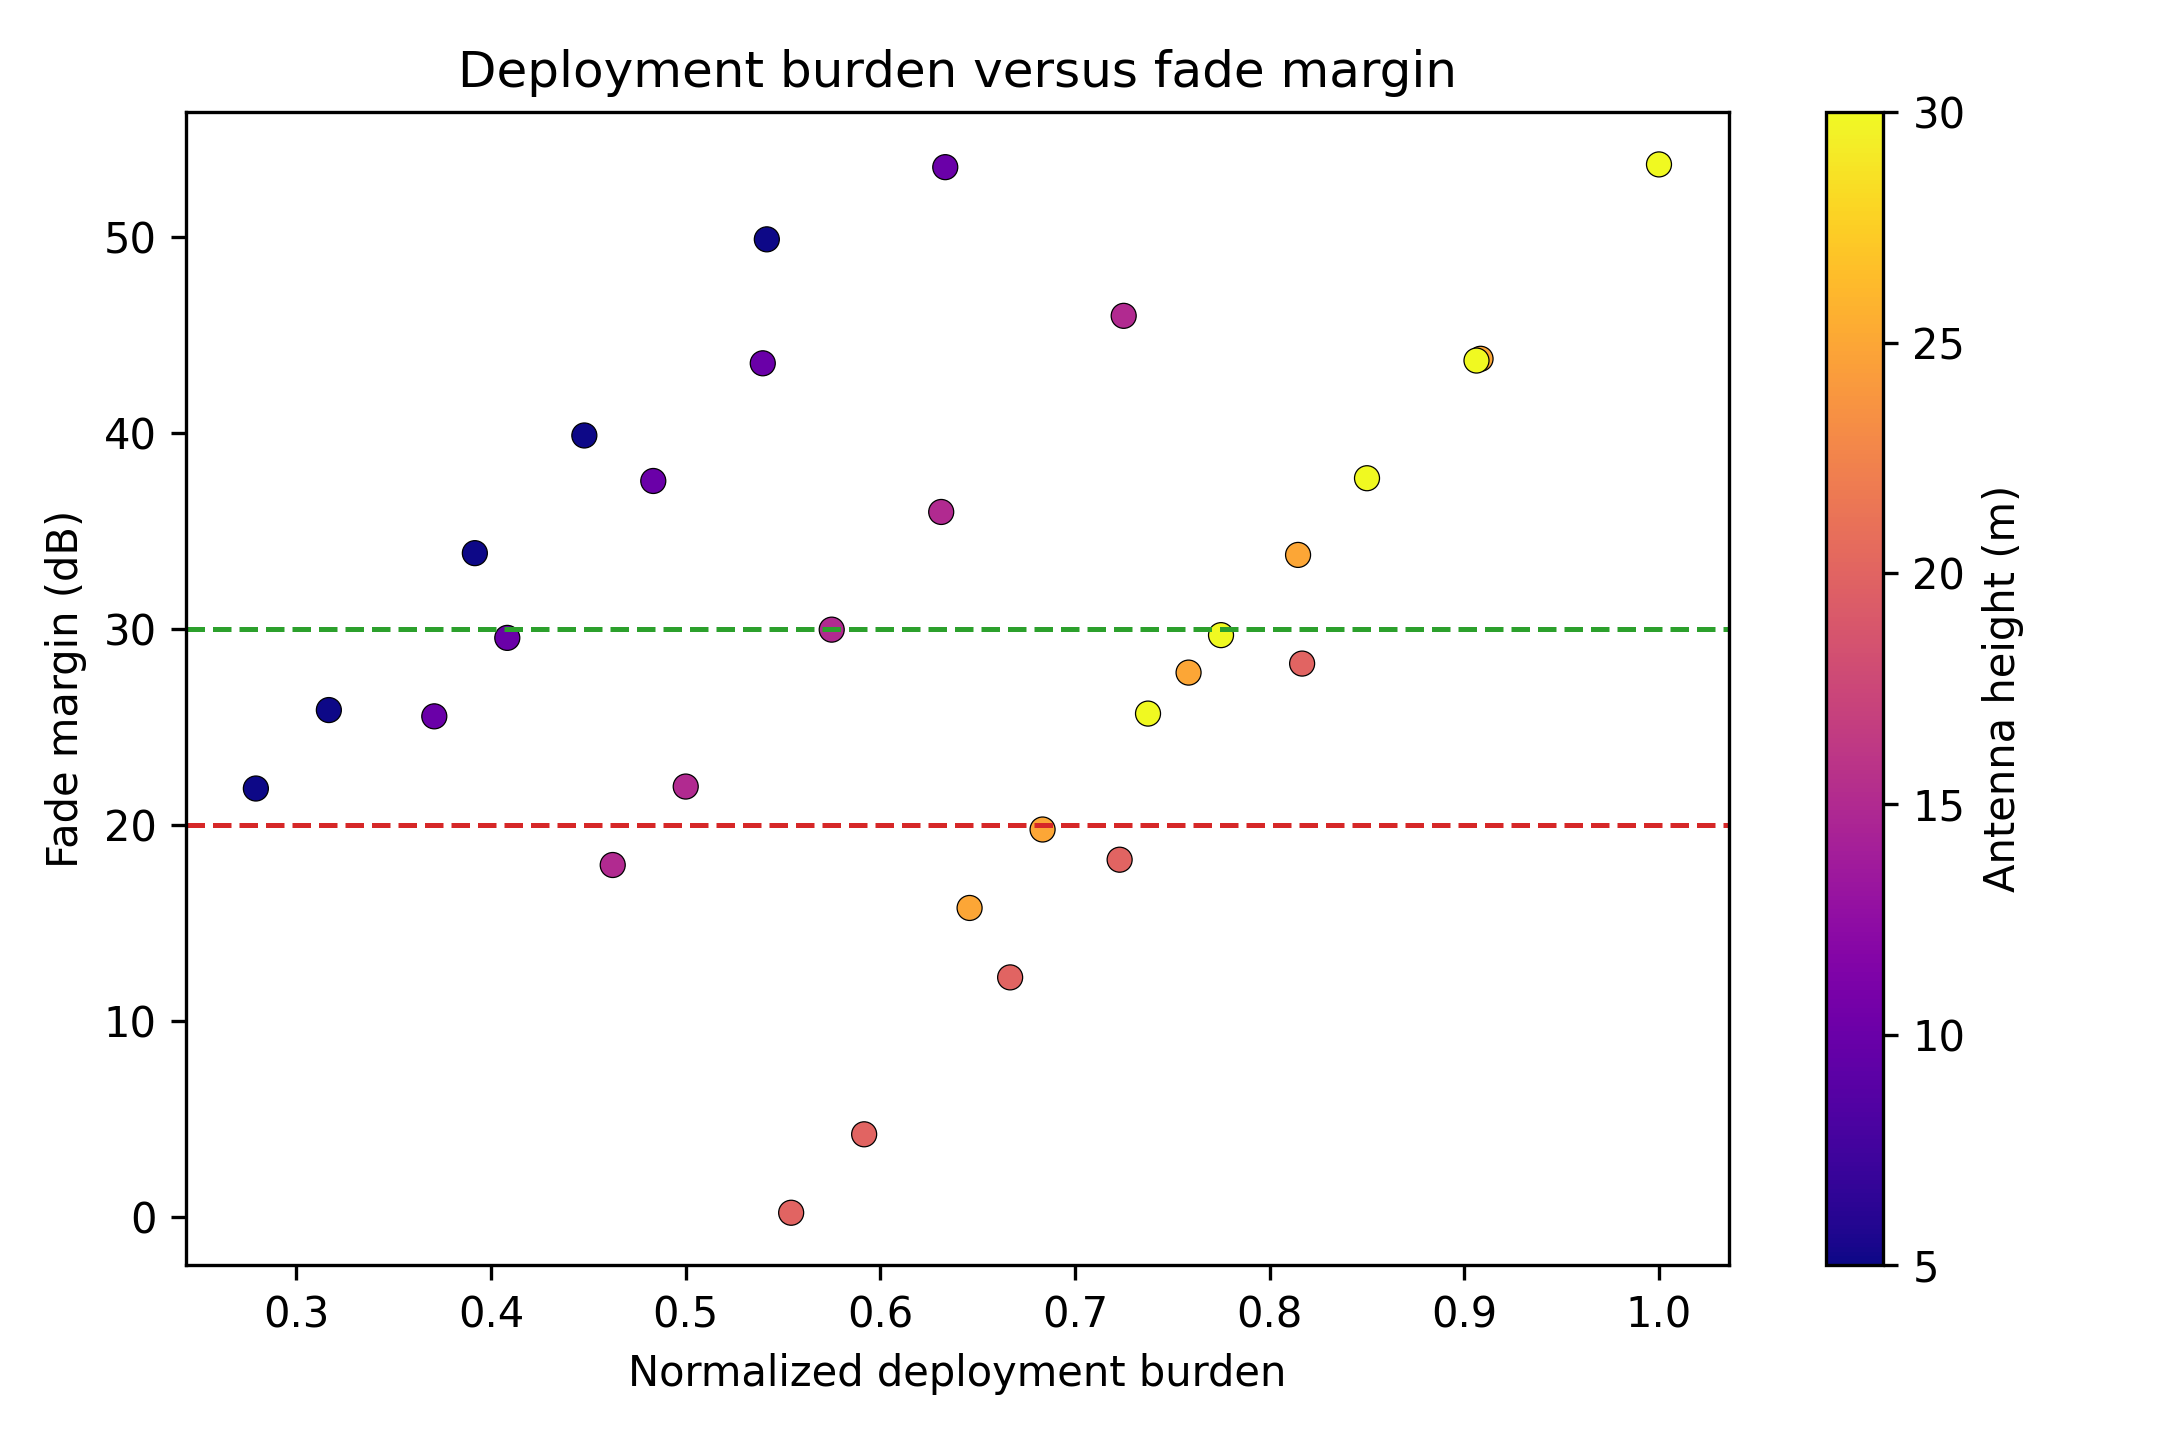
\includegraphics[width=\linewidth]{figures/cost_vs_fade_margin.png}
\caption{Normalized deployment burden versus Radio Mobile fade margin.}
\label{fig:cost}
\end{figure}

\section{Limitations}

The validation is against Radio Mobile, not against field measurements. The study uses one campus link, one accepted frequency, and symmetric antenna settings. The results should therefore be treated as a reproducible planning workflow and a site-specific case study. Additional links, field RSS measurements, and account-permitted lower-frequency simulations would be needed before making broader claims about regional deployment.

\section{Conclusion}

This paper developed and tested a terrain-aware planning model for a 5.8 GHz campus backhaul link. The 30-scenario Radio Mobile matrix showed that terrain obstruction can dominate the antenna-height decision. Height increases did not produce monotonic improvement; the 20 m case produced the weakest margins because Radio Mobile reported a 19.43 dB obstruction loss. The model comparison shows that FSPL alone is inadequate for this link, while a height-calibrated terrain/statistical correction closely matches the Radio Mobile outputs. For the studied deployment-burden objective, the recommended design is 5 m and 10 dBi for a 20 dB margin, or 5 m and 16 dBi for a 30 dB margin.

\section*{Data and Code Availability}

The data and analysis files used to produce the results in this paper should be shared in a public repository before submission. The reproducibility package includes the raw Radio Mobile HTML outputs for the 30 simulated scenarios, the processed CSV files, the validation summary, the Python analysis script, and the generated figures. In this project folder, these files are located under \texttt{data/}, \texttt{figures/}, and \texttt{analyze\_radio\_mobile\_results.py}. The main processed datasets are \texttt{radio\_mobile\_expanded\_results.csv}, \texttt{radio\_mobile\_expanded\_with\_model.csv}, and \texttt{validation\_metrics.csv}. After archiving the package, replace this sentence with the final repository citation and link, for example: ``Data and code are available at Zenodo: \url{https://doi.org/10.5281/zenodo.xxxxxxx}.''

\bibliographystyle{IEEEtran}
\bibliography{references}

\end{document}
